\chapter{联邦学习中的自适应本地差分机制}

\label{ch3}

\section{引言}
与传统的集中式深度学习相比,联邦学习通过分布式训练在一定程度上缓解了隐私泄漏的问题。然而,许多研究表明,攻击者仍然可以通过模型训练的梯度损害用户的隐私\upcite{ref48}。深度学习技术可以"记忆"模型中的训练数据信息,在这种情况下,敌方一旦通过白盒推理攻击或者黑盒推理攻击访问模型,就可以推演出客户端本地的训练数据。

在传统的集中式隐私保护方案中,数据管理者倾向于给每个用户的数据以相同的隐私预算。同样的隐私预算忽略了用户之间的差异。有些用户希望有更好的隐私保护。而有些用户对某些数据的隐私不敏感。在这种情况下,由于联邦学习模型是分布式结构,从一个大数据库到许多小数据库,所以对于每个用户来说。他们只需要关心他们自己的隐私。他们可以设置不同的隐私预算方案,而不是传统的统一分配,然后在最坏的的情况下注入噪音。

联邦学习模型的优化问题可以概括为ERM(经验风险最小化)问题\upcite{ref40}:
\begin{equation}\label{eq:ERM}
\arg \min _{\theta \in \mathcal{C}}\left(F(\theta):=\frac{1}{m} \sum_{i=1}^{m} F_{i}(\theta)\right)
\end{equation}

从隐私保护的角度讲,我们只要截断了从原始输入到输出,在其中加入一道隐私保护屏障,具体在哪一步截断则对应于不同的方法。差分隐私保护机器学习的方法具体有以下几种:
\begin{itemize}
	\item \textbf{输入扰动:} 输入扰动是在获取的训练数据上直接添加噪声,之后的模型训练和优化都是基于加躁后的训练数据\upcite{37}\upcite{38}\upcite{39}。
	\item \textbf{输出扰动:} 输出扰动沿袭了拉普拉斯机制最简单的思路,即考虑函数输出的敏感度来添加噪声,那么在ERM公式中我们只需要考虑argmin函数输出的敏感度,基于这个敏感度来添加拉普拉斯噪声即可得到一个简单的满足差分隐私的ERM方法\upcite{ref36}。
	\item \textbf{梯度扰动:} 梯度扰动是在执行最小化损失函数的过程中,设计满足差分隐私的算法。
	\item \textbf{目标扰动:} 目标扰动是在模型的目标函数中添加一个随机量,以使得最终模型的输出满足随机性。
\end{itemize}

基于输入的扰动和输出的扰动基本可以视为一个黑匣子模型,简单直接。但是这种添加噪声的方式无法对训练过程中数据的相互依赖性和输出有效性作出有用的、紧密的描述。在输入数据中加入过多的噪声,可能会影响模型训练的收敛性。在输出参数中加入过于保守的噪声,也就是根据最坏的攻击情况去添加噪声,可能会影响模型的实用性。

当前在深度学习模型中应用差分隐私的主流方案是在模型的梯度上添加噪声,方案的目标是在满足差分隐私的条件下,实现整体模型的最优可用性。Song等人\upcite{ref47}提出了一个$\left(\epsilon_{c}+\epsilon_{d}\right)$-差分隐私版本的随机梯度下降算法。在模型的每一次迭代过程中,对梯度添加高斯噪声,并通过差分隐私的组合性和隐私放大效果,得到完全隐私损失的上界。传统的联邦学习中使用差分隐私的主要流程如下所示:
\begin{itemize}
\item 本地计算:
客户端 $\mathrm{i}$ 根据本地数据库 $\mathcal{D}_{\mathrm{i}}$ 和接受的服务器的全局模型 $\mathrm{w}_{\mathrm{G}}^{\mathrm{t}}$ 作为本地的参数,即 $\mathrm{w}_{\mathrm{i}}^{\mathrm{t}}=\mathrm{w}_{\mathrm{G}}^{\mathrm{t}}$, 进 行梯度下降策略进行本地模型训练得到 $\mathrm{w}_{\mathrm{i}}^{\mathrm{t}+1} \quad(\mathrm{t}$ 表示当前通信回合) 。

\item 模型扰动:
每个客户端产生一个随机噪音 $\mathrm{n},\mathrm{n}$ 是符合高斯分布的,使用 $\overline{\mathbf{w}_{\mathrm{i}}}^{\mathrm{t}+1}=\mathrm{w}_{\mathrm{i}}^{\mathrm{t}+1}+\mathrm{n}$ 扰动本地模型 (这里注意w是一个矩阵,那么n就对矩阵的每一个元素产生噪音)。

\item 模型聚合:
服务器使用FedAVG算法聚合从客户端收到的 $\overline{\mathrm{w}}_{\mathrm{i}} \mathrm{t}+1$ 得到新的全局模型参数 $\mathrm{w}_{\mathrm{G}}^{\mathrm{t}+1}$, 也就是扰动过的模型参数。

\item 模型广播:
服务器将新的模型参数广播给每个客户端。

\item 本地模型更新:
每个客户端接受新的模型参数,重新进行本地计算。
\end{itemize}

然而,传统的基于差分隐私的联邦学习框架对所有本地数据添加相同的干扰,难免降低了全局模型的精度。因此本文采用一种更加复杂的方法来分析训练过程中训练数据对模型输出的贡献比率,然后根据每一层神经网络对模型输出的贡献率,在梯度上自适应添加噪声。

在本文中,我们认为中央参数服务器是半可信的(Honest but Curious, HbC),一个"诚实但好奇"的实体。也就是说,服务器将遵循与所有用户的协议。然而,通过利用完全访问用户梯度的便利,它也试图在训练过程中获得关于客户端的额外的信息。出于这个原因,我们的提出的自适应加噪机制目的是保护发送到服务器的本地梯度不被推断出任何关于用户的额外信息,并且尽量维持原有模型的精度。

总的来说,本章提出的隐私保护方案是基于本地客户端的本地数据维度的,从以下三个方面展开研究:第一,通过在本地模型训练的梯度下降算法过程中针对不同层的贡献比自适应添加噪声;第二,采用解析高斯机制,计算对其梯度施加的噪声大小;第三,使用差分隐私的组合定理和后处理定理分析模型整体的隐私性。

\section{基于自适应差分隐私的随机梯度下降算法}

算法\ref{基于自适应差分隐私的随机梯度下降算法}详细描述了在本地客户端训练过程中,在SGD算法中添加自适应差分隐私,并使用解析高斯机制衡量所添加的噪声大小。首先,我们采用先验组合机制计算$eps_{iter}$和$\delta_{iter}$(算法第7行)。每个客户端对训练数据进行采样,并计算他们的隐私预算$\delta_{u}$。如果$\delta_{u}>\delta$,用户将终止采样和训练,并且不上传其梯度信息(算法第9-12行)。否则,用户将计算梯度的贡献率(算法第16行),接着使用拉普拉斯机制注入自适应的噪声量(算法第18行),然后对梯度进行范数裁剪(算法第19行)。最后,服务器对用户的梯度进行平均,并更新模型参数$w$。该算法有三个主要部分:自适应差分隐私,梯度范数裁剪,以及采用解析高斯计算累积添加的噪声量。

\begin{algorithm}[!htb]
	\caption{基于自适应差分隐私的随机梯度下降算法}
	\label{基于自适应差分隐私的随机梯度下降算法}
	\begin{algorithmic}[1]
		\footnotesize
		\STATE \textbf{输入:} 预估迭代次数$T$,学习率$\alpha$,梯度裁剪阈值$C$,目标损失函数$l$,解析高斯机制噪声$(\Delta, \varepsilon, \delta)$,$f$贡献率阈值,$p$注入噪声的概率
		\STATE \textbf{输出:} 模型梯度
		\STATE 初始化模型权重$w$
		\WHILE{$\exists \delta_{u}<\delta$}
			\STATE $n$=0
			\STATE $grad$=0
			\STATE 计算$eps_{iter}$,$\delta_{iter}$
			\FOR {each $u \in$ Users}
				\STATE 计算$\delta_{u}$
				\IF{$\delta_{u}>\delta$}
					\STATE continue
				\ENDIF
				\STATE 从客户端数据集中随机采样
				\STATE $g t_{u}=\nabla l(w, x)$
				\STATE 计算梯度的平均贡献率
				\STATE $C_{j}\left(x_{i}\right)=\frac{1}{n} \sum_{i=1}^{n} C_{x_{i, j}}\left(x_{i}\right), j \in[1, u]$
				\STATE 添加自适应噪声
				\STATE $g t_{u}^{\prime}=g t_{u}+\frac{1}{\left|D_{i}^{t}\right|} \operatorname{Lap}\left(\frac{G S_{l}}{\epsilon_{j}}\right)$
				\STATE $g t_{u}=g t_{u} / \max \left(1, \frac{\left\|g t_{u}\right\|}{C}\right)$
				\STATE $n$++
			\ENDFOR
			\STATE $w=w-\alpha * g r a d / n$
		\ENDWHILE
	\end{algorithmic}
\end{algorithm}

\section{详细设计}
在本节接下来的三个部分,我们将详细描述如何在神经网络的随机梯度下降算法中自适应添加噪声、梯度剪裁以及使用解析高斯机制衡量添加的噪声大小。

\subsection{自适应噪声添加}
在第二章我们详细介绍了深度神经网络的结构,每个用户在本地用原始数据进行训练,在神经网络中进行前向传播操作,得到本地模型的输出。输入层的前向传播是神经网络中前向传播算法的第一步。

\begin{figure}[!hbt]
\centering
	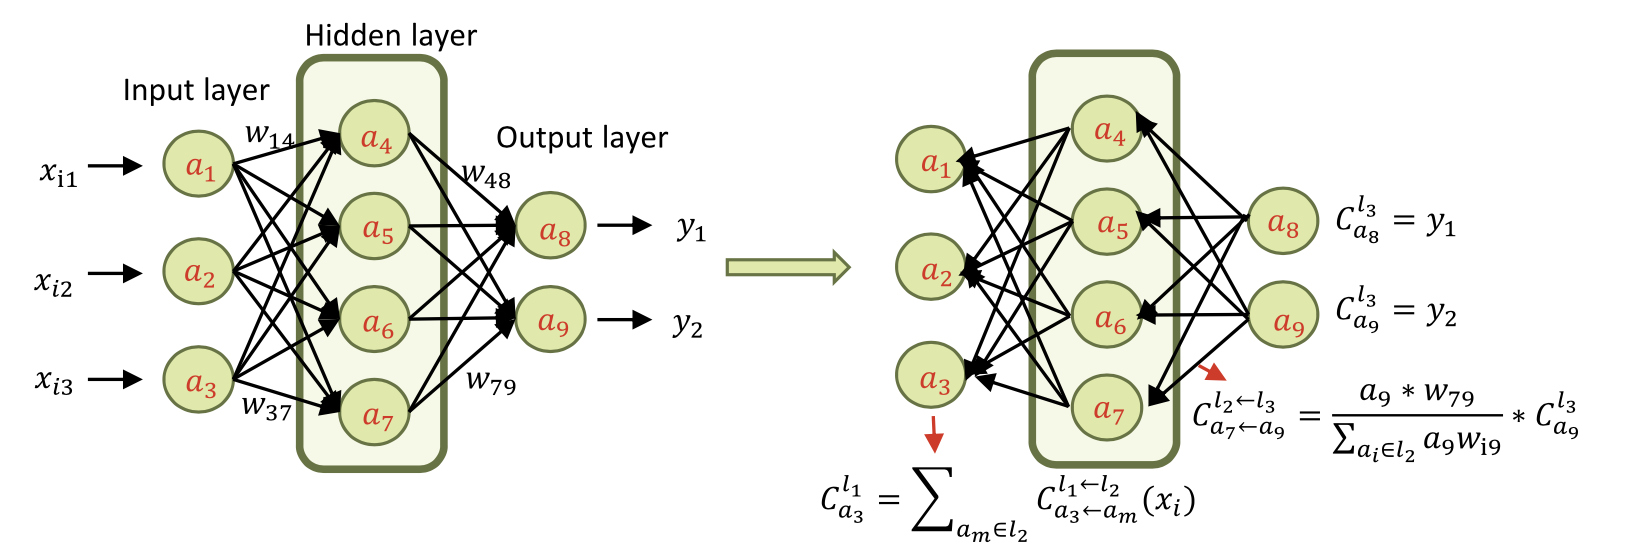
\includegraphics[scale=0.5]{fig2/C3/前向传播算法}%联邦学习的系统架构
	\caption{层间依赖传播算法}
	\label{fig:层间依赖传播算法}	
\end{figure}

我们采用层间相关性传播算法计算每一层对模型输出的贡献比率。每个用户都在本地对原始数据在神经网络中进行前向传播的训练,这可以获得一个新的数据操作,从而获得本地模型的输出。

"$\leftarrow$"表示两部分之间的连接关系。"$l_{2} \leftarrow l_{3}$" 是指深度神经网络中第2层和第3层之间相邻层的连接关系。
当第k层为输出层时,我们有:
\begin{equation}
C_{a_{i}}^{l_{k}}\left(x_{i}\right)=f\left(x_{i}, \omega_{i}^{r}\right)
\end{equation}

根据矩阵层之间的线性相关性,神经元$a_{i}$在第k层的贡献$C_{a_{i}}^{l_{k}}\left(x_{i}\right)$等于连接到神经元$a_{i}$的相邻层的贡献之和:
\begin{equation}\label{eq:层间传播1}
C_{a_{i}}^{l_{k}}\left(x_{i}\right)=\sum_{a_{j} \in l_{k+1}} C_{a_{i} \leftarrow a_{j}}^{l_{k} \leftarrow l_{k+1}}\left(x_{i}\right)
\end{equation}

比如,在图\ref{fig:层间依赖传播算法}中,存在:
\begin{equation}\label{eq:层间传播2}
C_{a_{7}}^{l_{2}}\left(x_{i}\right)=\sum_{a_{j} \in l_{3}} C_{a_{7} \leftarrow a_{j}}^{l_{2} \leftarrow l_{3}}\left(x_{i}\right)=C_{a_{7} \leftarrow a_{8}}^{l_{2} \leftarrow l_{3}}\left(x_{i}\right)+C_{a_{7} \leftarrow a_{9}}^{l_{2} \leftarrow l_{3}}\left(x_{i}\right)
\end{equation}

因此,神经元$a_{j}$对于输出层的贡献等于模型的输出。第k层的神经元$a_{j}$对于第k-1层的神经元$C_{a_{i} \leftarrow a_{j}}^{l_{k-1} \leftarrow l_{k}}\left(x_{i}\right)$等于:
\begin{equation}
C_{a_{i} \leftarrow a_{j}}^{l_{k-1} \leftarrow l_{k}}\left(x_{i}\right)=\left\{\begin{array}{cc}\frac{a_{i} w_{i, j}}{\sum_{a_{i} \in l_{k-1} a_{i} w_{i, j}}} C_{a_{j}}^{l_{k}}\left(x_{i}\right) & \sum_{a_{i} \in l_{k-1}} a_{i} w_{i, j} \neq 0 \\ \mu & \sum_{a_{i} \in l_{k-1}} a_{i} w_{i, j}=0\end{array}\right.
\end{equation}

其中$\mu$是一个无限接近于零,但大于零的数字。从上述公式中,我们可以认为每一层的贡献是相等的,而且贡献是逐层传递的。根据以上公式的推导,我们能得到神经网络模型中每一层以及每个神经元的贡献值。

通过从数据元组中提取同一属性的贡献,我们可以计算出每个属性类对模型输出的平均贡献:
\begin{equation}\label{eq:属性添加自适应扰动}
C_{j}\left(x_{i}\right)=\frac{1}{n} \sum_{i=1}^{n} C_{x_{i, j}}\left(x_{i}\right), j \in[1, u]
\end{equation}

在原始的参数上计算神经网络中每个属性类对于模型输出的贡献后,按照公式\ref{eq:属性添加自适应扰动-拉普拉斯机制}采用拉普拉斯机制在属性类的贡献率中注入噪音以保护原始的参数。
\begin{equation}\label{eq:属性添加自适应扰动-拉普拉斯机制}
\ddot{C}_{j}\left(x_{i}\right)=C_{j}\left(x_{i}\right)+\operatorname{Lap}\left(\frac{G S_{c}}{\epsilon_{c}}\right), j \in[1, u]
\end{equation}
其中,函数的局部敏感度为$G S_{c}=\frac{2 u}{|D|}$,$u,|D|$分别代表了属性和数据元组的最大数量。

在第二章中我们介绍了关于神经网络的结构,
\begin{equation}\label{eq:神经网络参数传递}
y=a(\mathbf{x} * \omega+b)
\end{equation}

公式\ref{eq:神经网络参数传递}表示学习模型中每个隐藏神经元的转化过程。
其中$\mathbf{x}$代表输入向量,$y$是输出,$b$和$\omega$分别代表{}偏置项和权重矩阵。$a()$是一个激活函数,用于结合线性变换和非线性变换。$y=a(\mathbf{x} * \omega+b)$ 是线性变换部分。

由于神经网络的结构,上一层的输出是下一层的输入,由此我们可以得出,原始的训练数据只被第一隐层的线性变换所利用。直观地说,为了得到一个具有隐私保护的学习模型,我们可以在第一层隐藏层的数据中注入噪声。正如Phan等人\upcite{ref36}提到的,对于线性变换有一种传统的方法,即向原始数据注入具有相同隐私预算的噪声,但是这容易导致隐私预算增加,并且使原始数据失真过多。因此,本文提出一种自适应噪声添加算法,针对每个梯度计算其贡献值,根据贡献值进行梯度裁剪并添加噪声。

首先,我们引入了两个调整因素$f$和$p$。其中,$f$代表一个阈值,用于决定属性对模型结果输出的贡献是高还是低,其值由用户定义,即贡献超过阈值$f$的属性类对输出的贡献更大。然后,我们向所有这些属性注入自适应拉普拉斯噪声。当贡献率低于阈值$f$时,对这些属性进行概率选择。也就是说,我们选择概率为$1-p$的原始数据,并对一些概率为$p$的属性注入自适应拉普拉斯噪声。该公式如下:
\begin{equation}\label{eq:神经网络加噪}
\tilde{x}_{i, j}=\left\{\begin{array}{ll}
\ddot{x}_{i, j} & \beta \geq f \\
\bar{x}_{i, j} & \beta<f
\end{array}\right.
\end{equation}

其中$\beta$代表贡献率:$\beta=\frac{\left|\ddot{C}_{j}\right|}{\sum_{j=1}^{u}\left|\ddot{C}_{j}\right|}$,当$\beta<f$时,我们有:
\begin{equation}\label{eq:神经网络加噪2}
\bar{x}_{i, j}=\left\{\begin{array}{l}
\ddot{x}_{i, j} \text { with probability } p \\
x_{i, j} \text { with probability } 1-p
\end{array}\right.
\end{equation}


$f$和$p$是超参数,用户可以根据自己的情况来调整。

也就是说,隐私预算$\epsilon_{l}$是根据贡献率:$\epsilon_{j}=\frac{u *\left|\ddot{C}_{j}\right|}{\sum_{j=1}^{u}\left|\ddot{C}_{j}\right|} * \epsilon_{l}$按比例分配给每个属性类,自适应噪声按以下方式注入属性中:
\begin{equation}\label{eq:神经网络加噪3}
x_{i, j}^{\prime}=x_{i, j}+\frac{1}{\left|D_{i}^{t}\right|} \operatorname{Lap}\left(\frac{G S_{l}}{\epsilon_{j}}\right)
\end{equation}

在不丧失一般性的情况下,调整因子$f$和$p$的值与系统的准确性和隐私水平有关。即$f$越小,$p$越大。越高的秘密水平,准确性越低,反之亦然。当f值为0.15,p设置为0.85时,使用自适应的噪声分布与拉普拉斯机制基本吻合。我们可以得出一个令人信服的结论,在相同的噪声水平下,自适应噪声添加的隐私预算接近于原始的拉普拉斯机制,因此我们的方案在缩小调整系数范围的情况下能达到相近的隐私保护效果。

\subsection{梯度范数裁剪}
在模型的每一轮迭代过程中,算法将计算添加了拉普拉斯噪声的梯度$g t_{u}^{\prime}=g t_{u}+\frac{1}{\left|D_{i}^{t}\right|} \operatorname{Lap}\left(\frac{G S_{l}}{\epsilon_{j}}\right)$, 方差是 $2 b^{2}$ 。对梯度注入的噪声量$\frac{1}{\left|D_{i}^{t}\right|} \operatorname{Lap}\left(\frac{G S_{l}}{\epsilon_{j}}\right)$,决定于用户个体对于梯度 $g$ 在二范数下的最大全局敏感度, 即$\delta$ 。由于梯度的大小没有一个先验的界限, 我们采用二范数的固定值对每个梯度进行裁剪。

用户上传的梯度向量将可以改写为$g t_{u}=g t_{u} / \max \left(1, \frac{\left\|g t_{u}\right\|}{C}\right)$, 其中 $C$是裁剪阈值。对于梯度的裁剪能保证梯度值小于设定的阈值$\mathrm{i}$。 也就是当 $\|g\| \leq C$ ,$g$ 保持不变;当$\|g\|>C$ 时, 它会按照裁剪比例缩小为 $C_{\circ}$。

但是如果裁剪阈值$C$ 的值如果太小,那么裁剪后的噪声会较小,算法添加的噪声较小时可能会破坏梯度估计的无偏性;可是如果不对梯度进行裁剪,大量的噪声添加到每个梯度会导致模型的可用性大大降低。在模型训练前期,梯度所包含的数据信息更多,因此可以对应添加更多的高丝噪声,使用较大的$C$ 的值,使得梯度裁剪后的模型偏差更小;而在模型训练后期,梯度所包含的数据信息相对较小了,如果还使用相同的$C$ ,会引入很多不必要的噪声。

因此我们根据训练轮数和层间贡献率动态调整梯度裁剪阈值$C$:在每次迭代中,该算法使用方差为$2 b^{2}$ 的拉普拉斯机制来计算噪声梯度$g t_{u}^{\prime}=g t_{u}+\frac{1}{\left|D_{i}^{t}\right|} \operatorname{Lap}\left(\frac{G S_{l}}{\epsilon_{j}}\right)$。噪声$2 b^{2}$ 的大小取决于一个个体在$l_{2}$规范下对$g$的最大影响,即$\delta$。由于对梯度的大小没有先验的约束,我们以$l_{2}$规范对每个梯度进行剪辑。因此,梯度向量$g$被$g t_{u}=g t_{u} / \max \left(1, \frac{\left\|g t_{u}\right\|}{C}\right)$取代,以达到剪裁阈值$C$。这种剪裁保证了如果$|g t_{u}\| \leq C$,那么$g t_{u}$将被保留,而如果$|g\|>C$,它将被裁减为梯度准则$C$。

\subsection{解析高斯机制}
在第二章的基础知识中, 我们简要介绍了传统的高斯机制。它的定义如下: 
\begin{define}\label{差分隐私高斯机制}
对于任意 $\varepsilon \in(0,1)$ 与 $c^{2}>2 \ln (1.25 / \delta)$, 高斯噪声参数满足 $\sigma \geq c \Delta_{2} f / \varepsilon$ 的高斯干扰机制为 $(\varepsilon, \delta)$-差分隐私。
\end{define}

在此基础上我们自然的有两个疑问:一是是否定义中的参数 $\sigma$ 是使算法满足 $(\varepsilon, \delta)$-差分隐私的最小值, 即是否可以施加更小的干扰来达到相同的差分隐私保护效果; 二是如果隐私预算 $\varepsilon$ 大于 1 会发生什么。

Balle\upcite{ref44}等人分析了传统的高斯机制在高隐私保护力度、隐私损失分析、低隐私保护力度三个方面中存在的问题,提出了一种改进的解析高斯机制(Analytic Gaussian Mechanism )。传统的高斯机制施加的噪声干扰过大, 方差公式在高隐私预算下过紧, 并且无法适用于隐私预算大于 1 的低隐私保护力度场景。解析高斯机制针对这些局限性提出了解决方案。

解析高斯机制的核心思想是使用高斯累积分布函数的计算, 来代替传统高斯机制的尾部约束近似。它的定义如下:
\begin{define}\label{解析高斯机制}
令 $f: \mathbb{N}^{\mathbb{N}^{\prime}} \rightarrow \mathbb{R}^{d}$ 表示一个 $\ell_{2}$ 敏感度为 $\Delta_{2}$ 的函数, 对任意 $\varepsilon \geq 0$ 与 $\delta \in[0,1]$, 当且仅当 $\sigma$ 满足下列不等式时, 含参数 $\sigma$ 的高斯机制满足 $(\varepsilon, \delta)$-差分隐私:
\begin{equation}\label{eq:解析高斯机制}
\Phi\left(\frac{\Delta_{2}}{2 \sigma}-\frac{\varepsilon \sigma}{\Delta_{2}}\right)-e^{\varepsilon} \Phi\left(-\frac{\Delta_{2}}{2 \sigma}-\frac{\varepsilon \sigma}{\Delta_{2}}\right) \leq \delta
\end{equation}
\end{define}

其中, $\Phi(t)=(1+\operatorname{erf}(t / \sqrt{2})) / 2$, erf 是高斯误差函数, 即 $\operatorname{erf}(x)=\frac{2}{\sqrt{\pi}} \int_{0}^{x} e^{-\eta^{2}} d \eta$ 。传统的差分隐私高斯机制的干扰大小$\sigma$可以直接计算,解析高斯机制的实现如下算法:

\begin{algorithm}[!htb]
	\caption{解析高斯算法}
	\label{解析高斯算法}
	\begin{algorithmic}[1]
		\footnotesize
		\STATE \textbf{输入:} $f, x, \Delta, \varepsilon, \delta$
		\STATE \textbf{输出:} 干扰后的 $f$
		\STATE 令 $\delta_{0}=\Phi(0)-e^{\varepsilon} \Phi(-\sqrt{2 \varepsilon})$
		\IF{如果 $\delta \geq \delta_{0}$}
			\STATE 定义 $B_{\varepsilon}^{+}(v)=\Phi(\sqrt{\varepsilon v})-e^{\varepsilon} \Phi(-\sqrt{\varepsilon(v+2)})$
			\STATE 计算 $v^{*}=\sup \left\{v \in \mathbb{R}_{\geq 0}: B_{\varepsilon}^{+}(v) \leq \delta\right\}$
            \STATE 令 $\alpha=\sqrt{1+v^{*} / 2}-\sqrt{v^{*} / 2}$
        \ELSE
        	\STATE 定义 $B_{\varepsilon}^{-}(u)=\Phi(-\sqrt{\varepsilon u})-e^{\varepsilon} \Phi(-\sqrt{\varepsilon(u+2)})$
        	\STATE 计算 $u^{*}=\inf \left\{u \in \mathbb{R}_{\geq 0}: B_{\varepsilon}^{-}(u) \leq \delta\right\}$
        	\STATE 令 $\alpha=\sqrt{1+u^{*} / 2}+\sqrt{u^{*} / 2}$
        \ENDIF
    	\STATE 令 $\sigma=\alpha \Delta / \sqrt{2 \varepsilon}$
    	\STATE \textbf{输出:} $f(x)+\mathcal{N}\left(0, \sigma^{2} I\right)$
	\end{algorithmic}
\end{algorithm}


\section{隐私性证明}
自适应差分SGD算法对线性变换函数进行了扰动,该函数满足$\left(\epsilon_{c}+\epsilon_{l}\right)$差分隐私。证明如下:

在贡献中添加的扰动为:
\begin{equation}\label{eq:贡献中添加的噪声}
\ddot{C}_{j}\left(x_{i}\right)=C_{j}\left(x_{i}\right)+\operatorname{Lap}\left(\frac{G S_{c}}{\epsilon_{c}}\right), j \in[1, u]
\end{equation}
它是满足$\epsilon_{c}$-差分隐私的。

贡献$G S_{c}$的敏感度为:
\begin{equation}\label{eq:贡献敏感度}
\begin{aligned}
G S_{c} &=\frac{1}{|D|} \sum_{j=1}^{u}\left\|\sum_{x_{i} \in D} C_{x_{i, j}}\left(x_{i}\right)-\sum_{x_{i}^{\prime} \in D^{\prime}} C_{x_{i, j}^{\prime}}\left(x_{i}^{\prime}\right)\right\|_{1} \\
&=\frac{1}{|D|} \sum_{j=1}^{u}\left\|C_{x_{n, j}}\left(x_{n}\right)-C_{x_{n, j}^{\prime}}\left(x_{n}^{\prime}\right)\right\|_{1} \\
& \leq \frac{2}{|D|} \max \sum_{j=1}^{u}\left\|C_{x_{i, j}}\left(x_{i}\right)\right\|_{1} \\
& \leq \frac{2 u}{|D|}
\end{aligned}
\end{equation}

其中,$u$和$|D|$分别表示贡献的数量和元组,然后可以得到:
\begin{equation}\label{贡献数量和元组}
\begin{aligned}
\frac{\operatorname{Pr}(\ddot{C}(D))}{\operatorname{Pr}\left(\ddot{C}\left(D^{\prime}\right)\right)} &=\frac{\prod_{j=1}^{u} \exp \left(\frac{\epsilon_{c}\left\|\frac{1}{|D|} \sum_{x_{i} \in D} C_{j}\left(x_{i}\right)-\ddot{C}_{j}\left(x_{i}\right)\right\|_{1}}{G S_{c}}\right)}{\prod_{j=1}^{u} \exp \left(\frac{\epsilon_{c}\left\|\frac{1}{\left|D^{\prime}\right|} \sum_{x_{i}^{\prime} \in D^{\prime}} C_{j}\left(x_{i}^{\prime}\right)-\ddot{C}_{j}\left(x_{i}^{\prime}\right)\right\|_{1}}{G S_{c}}\right)} \\
&=\prod_{j=1}^{u} \exp \left(\frac{\epsilon_{c}}{|D| G S_{c}}\left\|C_{j}\left(x_{n}\right)-C_{j}\left(x_{n}^{\prime}\right)\right\|_{1}\right) \\
& \leq \prod_{j=1}^{u} \exp \left(\frac{\epsilon_{c}}{|D| G S_{c}} \max \left\|C_{j}\left(x_{n}\right)\right\|_{1}\right) \\
&=\exp \left(\epsilon_{c} \frac{\max _{x_{i} \in D} \sum_{j=1}^{u}\left\|C_{j}\left(x_{n}\right)\right\|_{1}}{|D| G S_{c}}\right) \\
& \leq \exp \left(\epsilon_{c}\right)
\end{aligned}
\end{equation}

因此,添加噪声后的贡献值是满足$\epsilon_{c}$-差分隐私的。

假设两个相邻的批次$D_{i}^{t}$和$D_{i}^{t^{\prime}}$,其最后一个元组$x_{n}$和$x_{n}^{\prime}$不同,$z\left(D_{i}^{t}\right)$和$z\left(D_{i}^{t^{\prime}}\right)$分别为线性变换函数。

一般来说,我们把偏置项视为第一类数据属性,即:$x_{i,0}=b_{i}$。线性转换可以改写为:$\ddot{\mathbf{z}}_{x \in D_{i}^{t}}(\omega)=\ddot{\mathbf{x}} * \omega$。线性变换的敏感性$G S_{l}$如下:
\begin{equation}
\begin{aligned}
G S_{l} &=\sum_{a_{i} \in l_{1}} \sum_{j=1}^{u}\left\|\sum_{x_{i} \in D_{i}^{t}} x_{i, j}-\sum_{x_{i}^{\prime} \in D_{i}^{t^{\prime}}} x_{i, j}^{\prime}\right\|_{1} \\
&=\sum_{a_{i} \in l_{1}} \sum_{j=1}^{u}\left\|x_{n, j}-x_{n, j}^{\prime}\right\|_{1} \\
& \leq \sum_{a_{i} \in l_{1}} \sum_{j=1}^{u} \max _{x_{i} \in D_{i}^{t}}\left\|x_{n, j}\right\|_{1} \\
& \leq \sum_{a_{i} \in l_{1}} u
\end{aligned}
\end{equation}

其中,$a_{i} \in l_{1}$是指第一隐藏层$l_{1}$中的神经元$a_{i}$,$u$是数据元组$x_{i} \in D_{i}^{t}$中的属性数。它包括两个调整因素:$f$和$p$,它们可以过滤多余的噪声。之后的属性的一般表达式如下:
\begin{equation}
\begin{aligned}
\tilde{x}_{i, j} &=[(1-f)+f * p] * \ddot{x}_{i, j}+f *(1-p) * x_{i, j} \\
&=[(1-f)+f * p]\left[x_{i, j}+\operatorname{Lap}\left(\frac{G S_{l}}{\epsilon_{j}}\right)\right]+[f *(1-p)] x_{i, j} \\
&=x_{i, j}+[(1-f)+f * p]\left[\operatorname{Lap}\left(\frac{G S_{l}}{\epsilon_{j}}\right)\right]
\end{aligned}
\end{equation}
然后我们可以得到:

\begin{equation}
\begin{aligned}
\frac{\operatorname{Pr}\left(\ddot{\mathbf{z}}_{D_{i}^{t}}(\omega)\right)}{\operatorname{Pr}\left(\ddot{\mathbf{z}}_{D_{i}^{t}}(\omega)\right)} &=\frac{\prod_{a_{i} \in l_{1}} \prod_{j=1}^{u} \exp \left(\frac{\epsilon_{j}\left\|\sum_{x_{i} \in D_{i}^{t}} x_{i, j}-\sum_{x_{i} \in D_{i}^{t}} \tilde{x}_{i, j}\right\|_{1}}{G S_{l}}\right)}{\prod_{a_{i} \in l_{1}} \prod_{j=1}^{u} \exp \left(\frac{\epsilon_{j}\left\|\sum_{x_{i}^{\prime} \in D_{i}^{t^{\prime}}} x_{i, j}^{\prime}-\sum_{x_{i}^{\prime} \in D_{i}^{t^{\prime}}} \tilde{x}_{i, j}^{\prime}\right\|_{1}}{G S_{l}}\right)} \\
& \leq \prod_{a_{i} \in l_{1}} \prod_{j=0}^{u} \exp \left(\frac{\epsilon_{j}}{G S_{l}}\left\|\sum_{x_{i} \in D_{i}^{t}} x_{i, j}-\sum_{x_{i}^{\prime} \in D_{i}^{t^{\prime}}} x_{i, j}^{\prime}\right\|_{1}\right) \\
& \leq \prod_{a_{i} \in l_{1}} \prod_{j=0}^{u} \exp \left(\frac{\epsilon_{j}}{G S_{l}} \max _{x_{i} \in D_{i}^{t}}\left\|x_{n, j}\right\|_{1}\right) \\
& \leq \exp \left(\epsilon_{l} \frac{\sum_{a_{i} \in l_{1}} u\left[\sum_{j=1}^{u} \frac{\left|\ddot{C}_{j}\right|}{\sum_{j=1}^{u}\left|\ddot{C}_{j}\right|}\right]}{G S_{l}}\right) \\
&=\exp \left(\epsilon_{l}\right)
\end{aligned}
\end{equation}

根据上述推倒证明可知,在联邦学习的神经网络中添加自适应噪声后,所上传的梯度是满足$\left(\epsilon_{c}+\epsilon_{l}\right)$差分隐私的。在满足差分隐私的基础上,在下一节我们会给出隐私损失累积函数计算隐私成本。

\section{隐私预算分析}
本章所提出的自适应差分隐私保护方案是通过在随机梯度下降算法上添加自适应的拉普拉斯扰动,保护数据的隐私性。在上一节我们已经证明了此算法满足$\left(\epsilon_{c}+\epsilon_{l}\right)$差分隐私,那另外一个非常重要的问题就是评估在训练过程中添加噪声所累积的隐私预算成本。在本节中,我们提出隐私损失累计函数的概念,去计算算法迭代过程中添加噪声所累积的隐私预算成本。

根据差分隐私的组成定理,被查询n次的数据的隐私风险将增加n倍。因此,我们希望查询次数越少越好,至少要有一个界限。在实验环境中,我们可以通过几次尝试确定一个相对理想的迭代次数,然后在每次迭代中平均分配隐私预算。然而,在实践中很难选择迭代的数量,因为任何尝试都会增加额外的隐私风险。当数量太小时,会发生预拟合,导致性能不佳;如果数量太大,注入的噪声会过大,这将影响模型的准确性。另一种尝试是使用等比例递增的注入噪声序列,这样无论我们有多少次迭代,我们都能找到有限的隐私预算\upcite{ref32}。

根据上文提出的解析高斯机制,结合差分隐私的组成定理,我们设计了一个解析高斯组成定理:
\begin{theorem}[解析高斯组成定理]\label{解析高斯组成定理}
假使存在算法$M_{i}$满足$\left(\varepsilon_{i}, \delta_{i}\right)$-差分隐私,那么对于$M_{[k]}=\left(M_{1}, M_{2}, \ldots, M_{k}\right)$,有$M_{[k]}$也是满足$(\varepsilon, \delta)$-差分隐私的,其中
$$
\delta=\sum_{i=1}^{k} B(i, k, p)\left[\Phi\left(\frac{H \sqrt{i}}{2 \sigma}-\frac{\varepsilon \sigma}{H \sqrt{i}}\right)-e^{\varepsilon} \Phi\left(-\frac{H \sqrt{i}}{2 \sigma}-\frac{\varepsilon \sigma}{H \sqrt{i}}\right)\right]
$$
\end{theorem}

我们采用朴素贝叶斯机制计算$\delta$可以得到:
\begin{equation}\label{eq:朴素贝叶斯}
\delta=\sum_{i=1}^{k} B(i, k, p)\left[\operatorname{Pr}\left[L_{d, d^{\prime}} * i>\varepsilon\right]-e^{\varepsilon} \operatorname{Pr}\left[L_{d^{\prime}, d} * i<-\varepsilon\right]\right]
\end{equation}

在此情况下,隐私损失变量$L_{M, d, d^{\prime}}$和$L_{M, d^{\prime}, d}$同时满足$N(\eta, 2 \eta)$分布,并且$\eta=$ $H^{2} / 2 \sigma^{2}$。因此可以采用解析高斯机制这样表达隐私预算损失:
\begin{equation}\label{eq:隐私预算计算1}
\begin{aligned}
& \operatorname{Pr}\left[L_{d, d^{\prime}} * i>\varepsilon\right]=\operatorname{Pr}[N(\eta i, 2 \eta i)>\varepsilon] \\
=& \operatorname{Pr}\left[N(0,1)>\frac{-\eta i+\varepsilon}{\sqrt{2 \eta i}}\right]=\operatorname{Pr}\left[N(0,1)<\frac{\eta i-\varepsilon}{\sqrt{2 \eta i}}\right] \\
=& \operatorname{Pr}\left[N(0,1)<\sqrt{\frac{\eta i}{2}}-\frac{\varepsilon \sigma}{\sqrt{2 \eta i}}\right]=\Phi\left(\frac{H \sqrt{i}}{2 \sigma}-\frac{\varepsilon \sigma}{H \sqrt{i}}\right)
\end{aligned}
\end{equation}

然后,可以计算得到隐私预算:
\begin{equation}\label{eq:隐私预算计算2}
\delta=\sum_{i=1}^{k} B(i, k, p)\left[\Phi\left(\frac{H \sqrt{i}}{2 \sigma}-\frac{\varepsilon \sigma}{H \sqrt{i}}\right)-e^{\varepsilon} \Phi\left(-\frac{H \sqrt{i}}{2 \sigma}-\frac{\varepsilon \sigma}{H \sqrt{i}}\right)\right]
\end{equation}

因为随着算法迭代次数$T$的增加,$\Phi\left(\frac{H \sqrt{T}}{2 \sigma}-\frac{\varepsilon \sigma}{H \sqrt{T}}\right)-e^{\varepsilon} \Phi\left(-\frac{H \sqrt{T}}{2 \sigma}-\frac{\varepsilon \sigma}{H \sqrt{T}}\right)$也在增加,因此可以计算得到:

\begin{equation}\label{eq:隐私预算计算3}
\begin{aligned}
& \sum_{i=1}^{T} B(i, T, p)\left[\operatorname{Pr}\left[L_{d, d^{\prime}} * i>\varepsilon\right]-e^{\varepsilon} \operatorname{Pr}\left[L_{d^{\prime}, d} * i<-\varepsilon\right]\right] \\
\leq & \sum_{i=1}^{T} B(i, T, p)\left[\operatorname{Pr}\left[L_{d, d^{\prime}} * T>\varepsilon\right]-e^{\varepsilon} \operatorname{Pr}\left[L_{d^{\prime}, d} * T<-\varepsilon\right]\right] \\
\leq & \operatorname{Pr}\left[L_{d, d^{\prime}} * T>\varepsilon\right]-e^{\varepsilon} \operatorname{Pr}\left[L_{d^{\prime}, d} * T<-\varepsilon\right]
\end{aligned}
\end{equation}

当隐私预算$\delta$相同时,$\sigma_{1} \leq \sigma_{2} \leq \sigma_{3}$。替换$\sigma=\alpha H \sqrt{T} / \sqrt{2 \epsilon}$,则有
\begin{equation}\label{eq:隐私预算计算4}
\Phi(\sqrt{\epsilon / 2}(1 / \alpha-\alpha))-e^{\varepsilon} \Phi(-\sqrt{\epsilon / 2}(1 / \alpha+\alpha)) \leq \delta
\end{equation}

因此,$\sigma_{1} \leq \sigma_{3}=O(\sqrt{T})$。与之前的工作相比,我们的隐私预算能够在相同的迭代次数$T$,更低的上紧界,达到满足$\left(\epsilon_{c}+\epsilon_{l}\right)$的差分隐私。

\section{本章总结}
联邦学习以分布式学习技术为基础,使参与者彼此通过一定的方式(如中心服务器)联合起来训练一个神经网络。在这个过程中,参与者不需要将自己的隐私数据暴露出来便可以参与协作训练,可以克服参与者本地数据集较小、数据样本比较单一、隐私泄露等缺点。虽然基本的分布式协作深度学习没有直接暴露参与者的隐私数据集,但是恶意攻击者仍然可以通过共享的参数等信息获得一定的隐私信息。 

本章详细介绍了如何在深度学习模型的随机梯度下降算法中添加自适应的拉普拉斯噪声。其中梯度下降作为一种常见的深度学习优化方法,在梯度上添加扰动是最早被提出、也是当前比较主流的差分隐私加噪方案之一。我们设计了一个自适应噪声添加的方案,在神经网络前向传播算法中,根据属性对于模型输出的贡献率注入不同隐私预算的噪声。与传统的注入噪声的方法相比,我们在相同的隐私保护程度下最大限度地提高了模型的准确性,并且证明了算法能满足$\left(\epsilon_{c}+\epsilon_{l}\right)$差分隐私。然后我们采用解析高斯机制计算对梯度施加的噪声量大小,分析了模型整体的隐私预算。

然而,在客户端的本地数据集添加的噪声只能保证本地数据的匿名性,不能够防止外部攻击者针对通信信道的攻击。如果客户端在每次迭代中同时上传了大量的权重更新,中央云服务器仍然可以将它们链接在一起,推导出参数信息。而且,当参与一次迭代的客户端数量达到上千人时,会导致聚合任务升级成一个高维任务,隐私预算暴增。因此,下一章我们对联邦学习模型框架进行了改进,在现有的联邦学习模型上新增混洗器,实现联邦学习框架的隐私安全,提高整体联邦学习模型的精度。

